\documentclass{article}
\usepackage[utf8]{inputenc}
\usepackage[T1]{fontenc}
\usepackage[ngerman]{babel}
\usepackage{lmodern}
\usepackage{microtype}
\usepackage{graphicx}
\usepackage{float}
\usepackage{subcaption}
\usepackage{hyphenat}
\usepackage{natbib}
\usepackage{url}
\usepackage{amsmath}
\usepackage{booktabs}
\usepackage{tikz}
\usetikzlibrary{shapes.geometric, arrows.meta, positioning}
\captionsetup[subfigure]{skip=2pt, justification=centering}
\usepackage{xcolor}
\definecolor{blue!50}{RGB}{50,100,200}
\definecolor{green!50}{RGB}{34,140,34}
\definecolor{orange!50}{RGB}{200,100,50}
\setlength{\parindent}{0pt}
\setlength{\parskip}{6pt plus 2pt minus 1pt}

\begin{document}

\title{KI-basierte IGRT mit 2D-bildgeführtem Dose Tracking täglicher
Conebeam-CTs zur Bewertung der Füllung von Rektum und Harnblase
bei definitiver Radiotherapie des Prostatakarzinoms}

\author{%
\begin{minipage}{\textwidth}
\centering
\small
Peter Rhone, Dipl.-Phys.\textsuperscript{1}, 
Saskia Spautz, MSc\textsuperscript{2,3,*},\\ 
Annika Schlamann, MD\textsuperscript{2,3}, 
Thomas Kuhnt, MD, Prof.\textsuperscript{2,3},\\ 
Franziska Nägler, MD\textsuperscript{2,3,**} \\[1ex]
\footnotesize\textsuperscript{1}Klinik für Strahlentherapie und Radioonkologie, Heinrich-Braun-Klinikum Zwickau, \\ 
\footnotesize\textsuperscript{2}Klinik und Poliklinik für Strahlentherapie, Universitätsklinikum Leipzig \\ 
\footnotesize\textsuperscript{3}Mitteldeutsches Krebszentrum (CCCG), Partnerstandort Leipzig \\ 
\footnotesize\textsuperscript{*}geteilte Erstautorschaft
\footnotesize\textsuperscript{**}Seniorautorin
\end{minipage}%
}
\maketitle 

\vspace{0.5cm}

\begin{abstract}
\noindent
\textbf{Hintergrund:} Es wird eine schnelle Methode zur automatischen Erkennung von
Harnblase und Rektum in täglichen Cone-Beam-CTs (kV-CBCTs) für die
bildgesteuerte Strahlentherapie (IGRT) vorgestellt. \\ \textbf{Methoden:}
Mediale sagittale Schnitte wurden mittels künstlicher Intelligenz (KI)
segmentiert, um die Füllungszustände von Rektum und Harnblase bei der definitiven
Radiotherapie des Prostatakarzinoms zu bewerten. \\ \textbf{Ergebnisse:} Das Modell
wurde mit Daten von 131 Patienten trainiert und validiert mit jeweils 5 kV-CBCTs
pro Patient. Die Ergebnisse zeigen eine hohe Segmentierungsleistung mit mittleren
Dice-Werten von 0,9149 ± 0,0852 für die Harnblase und 0,7848 ± 0,1641 für das
Rektum sowie Hausdorff-Distanzen von 9,1419 ± 9,0216 px (Harnblase) und 11,5230 ± 10,5643 px
(Rektum). \\ \textbf{Zusammenfassung:} Die KI-basierte Methode kann die
Überprüfung von Organfüllung effektiv und schnell automatisieren und bietet
Potenzial zur Verbesserung der Behandlungsqualität und Effizienz in der IGRT. \\
\textbf{Schlüsselworte:} Segmentierung, Risikoorgane, Deep Learning, 
Medizinische Bildgebung, Cone-Beam-CT, CBCT, Strahlentherapie, Bildgesteuerte
Strahlentherapie, Künstliche Intelligenz
\end{abstract}

\section{Einleitung}
Bei der definitiven Bestrahlung von Prostatakarzinomen niedrigen und mittleren
Risikos kann eine perkutane Radiotherapie in Normfraktionierung, moderater
Hypofraktionierung oder Ultrahypofraktionierung angewendet werden
\citep{numakura2023,junius2007,dimuzio2009}. Dabei wird eine
Gesamtdosis in tägliche Fraktionen verabreicht.

Interfraktionelle Variabilität durch Änderungen der Füllungszustände oder
Organbewegungen im Beckenbereich kann Organe at Risk (OARs) wie Harnblase und
Rektum unerwünscht hohen Dosen aussetzen, was die akute oder chronische Toxizität
erhöhen kann \citep{quantec,devlin2015}.

Um diese Toxizitäten zu minimieren, ist ein zentraler Schritt in der modernen
Strahlentherapie die Verifizierung der genauen Position der umliegenden
Risikoorgane (OARs) vor jeder Fraktion mittels bildgesteuerter Strahlentherapie
(IGRT) \citep{kupelian2007,wang2022}. Es gibt verschiedene Methoden zur IGRT, z.\,B.
Cone-Beam-CTs (CBCT) oder in die Prostata implantierte Fiducials (Goldmarker) in
Kombination mit planaren Röntgenbildern \citep{dang2018}. Die Verifizierung der
OAR-Füllungszustände ist jedoch nur mit CBCT möglich. Damit können variierende
Füllungen und Bewegungen berücksichtigt und korrigiert werden, etwa eine
unzureichend gefüllte Harnblase oder ein luftgefülltes Rektum, um das Einhalten
von Dosis-Constraints wie \( V_{65} < 50\% \) für die Harnblase sicherzustellen
\citep{wall2018}.

Online-adaptive Strahlentherapie passt täglich diese Veränderungen an, erfordert
jedoch erheblichen Zeit- und Personalaufwand (15–35 Minuten pro Fraktion mit
Facharzt und Medizinphysikexperten), was in Hochdurchsatz-Kliniken kaum umsetzbar
ist \citep{byrne2022}. Häufig wird daher nur ein Offline-Review durchgeführt, bei
dem Abweichungen erst nachträglich erkannt werden.

Inspiriert von Fortschritten in der medizinischen Bildsegmentierung, entwickeln
wir eine KI-basierte Methode zur Teilautomatisierung der online-adaptiven Therapie,
um die Füllung der Risikoorgane in täglichen CBCT-Aufnahmen effizienter zu
überwachen und die Behandlungsqualität zu verbessern \citep{antonelli2022}.

\section{Methoden}
Zwischen dem 01.07.2019 und dem 31.01.2024 wurden retrospektiv 131 Patienten mit
Prostatakarzinom niedrigen bis mittleren Risikos ausgewählt, die eine
definitive, moderat hypofraktionierte Radiotherapie (25 Fraktionen mit
simultan-integriertem Boost, 58–68 Gy) erhielten, in Anlehnung an das Schema von
\citep{dimuzio2009}. Einschlusskriterien waren cT1a–cT2b, PSA $\leq
20\,\text{ng/ml}$ und Gleason-Score $\leq 7$; Patienten mit Hochrisikoprofil
oder Fernmetastasen wurden ausgeschlossen. Eine schriftliche Einwilligung zur
anonymen Datenverwendung liegt vor.

Für jeden Patienten wurden ein Planungs-CT (PL-CT) und 5 kV-CBCTs aus dem
RayStation-System (Versionen 10B–12A) anonymisiert extrahiert \citep{zwart2022}.
Strukturen (Harnblase, Rektum) wurden manuell von einem Medizinphysiker
konturiert und von einem Facharzt überprüft. Ein selbst entwickeltes
Python-Programm (\textit{sqlite\_dicom2.py}) \citep{rhone_repo} konvertierte
DICOM-Daten in Volumina, extrahierte fünf mediale sagittale 2D-Schnitte pro
kV-CBCT – zentral durch die Symphyse sowie je zwei links und rechts – und
erstellte Binärmasken mittels des Point-in-Polygon-Algorithmus, um präzise
Konturen für Strukturen zu generieren, die die Schnittebene mehrfach
durchschneiden, wie es häufig beim Rektum der Fall ist \citep{salomon1978}. Die
Ausgaben (Patienten-ID, DICOM-Serie, Schnitte, Masken, Schnittnummer) wurden in
eine SQLite-Datenbank gespeichert. Ein zweites Programm
(\textit{sqlite\_viewer.py}) \citep{rhone_repo} ermöglichte visuelle Kontrolle
und Datenbereinigung.

Bilder wurden vorverarbeitet: ungewöhnliche Bildgrößen (z.B.\ 85x512 Pixel)
wurden ausgeschlossen, da sie auf abweichende kV-CBCT-Protokolle zurückzuführen
waren und nur die Standardgröße (88x512 Pixel) beibehalten wurde, um anatomische
Details zu erhalten. Die Pixelintensitäten wurden von den gespeicherten Werten
(0–8000) auf [0, 1] normalisiert, indem durch den Maximalwert (8000) dividiert
wurde \citep{stevens2020}.

Insgesamt entstanden 3508 Bilder für die Harnblase (129 Patienten) und 3311
Bilder für das Rektum (128 Patienten), basierend auf 5 sagittalen Schnitten pro
kV-CBCT. \footnote{Manipulierte Bildzahlen aufgrund von Datenbereinigung: Einige
Patienten hatten weniger als 5 nutzbare CBCTs oder Schnitte aufgrund
unvollständiger Strukturen.}

\subsection{Kreuzvalidierungsdesign}
Um eine robuste Abschätzung der Generalisierbarkeit zu gewährleisten und
Datenlecks durch patientenübergreifende Abhängigkeiten auszuschließen, wurde
die Datenbank erst in Trainings- (80\%) und Validierungssets (20\%) aufgeteilt, 
streng auf Patientenebene, um klinische Realbedingungen abzubilden, unter 
denen das Modell auf vollständig neue Patienten angewendet wird. 
Die 129 Patienten der Harnblasendatenbank und 128 Patienten der Rektumdatenbank
wurden aufgeteilt in Trainings- (80\%) und Validierungssets (20\%).
Für die Harnblase ergab das Trainingsset 103 Patienten (2808 Bilder) und das
Validierungsset 26 Patienten (707 Bilder). Für das Rektum waren es 102 Patienten im
Trainingsset (2646 Bilder) und 26 Patienten im Validierungsset (665 Bilder).

Eine \textbf{5-fache patientendisjunkte Kreuzvalidierung} wurde auf dem 
Trainingsset durchgeführt. Die Trainingspatienten wurden jeweils zufällig in 
fünf disjunkte Teilmengen
partitioniert, wobei durch \textbf{Stratifizierung nach Organvolumen}
sichergestellt wurde, dass alle Füllungszustände in jedem Fold proportional
vertreten waren. T-Test-Analysen bestätigten für alle Folds keine signifikanten
Volumenunterschiede zwischen Trainings- und Validierungssets (p > 0.05).

Zur Vermeidung von Verzerrungen durch nicht-informative Samples wurden vor der
Modellierung alle Bilder mit leeren GT-Masken ($\sum \text{Maske} = 0$) aus den
Datensätzen entfernt - wenn etwa das Organ nicht im Bild sichtbar war. 

\subsection{Modelltraining und Evaluation}
Ein U-Net-basiertes Convolutional Neural Network (CNN) \citep{ronneberger2015}
wurde mit PyTorch trainiert, um kV-CBCT-Bilder zu segmentieren
\citep{stevens2020}. Das Modell verarbeitet mittelsagittale CT-Schnitte (88x512
Pixel) und besteht aus einer Encoder-Decoder-Architektur mit Skip-Connections
(Abb. \ref{fig:unet}). Die Trainingsbilder wurden mit den in Tabelle
\ref{tab:augmentation} spezifizierten Techniken augmentiert, was 16848 Bilder
für die Harnblase und 15936 Bilder für das Rektum ergab.

Während der Validierung wurden für jedes Bild im Validierungsset folgende
Metriken berechnet: Dice-Koeffizient, Präzision, Recall und Hausdorff-Abstand.
Bei leeren Modellvorhersagen ($\sum \text{Vorhersage} = 0$) wurde der
Hausdorff-Abstand als \texttt{NaN} gewertet, um verzerrte Ergebnisse zu
vermeiden, während Dice, Präzision und Recall entsprechend der binären
Klassifikationslogik berechnet wurden. Die Ergebnisse auf dem Validierungsset 
wurden als Mittelwert ± Standardabweichung berichtet.
Zusätzlich wurden für jeden Fold die Vorhersage mit dem niedrigsten
Dice-Koeffizienten visuell analysiert, um systematische Fehlerquellen zu
identifizieren.

\begin{table}[H]
    \centering
    \small
    \begin{tabular}{cc}
      \toprule
      \textbf{Augmentation} & \textbf{Parameter} \\
      \midrule
      Rotation & $-10^\circ$ bis $10^\circ$ \\
      Horizontales Spiegeln & \textemdash \\
      Rauschen & Gaußsches Rauschen, Varianz: 0,001 \\
      Verzerrung & Scherung: $-0,1$ bis $0,1$ \\
      Skalierung & $0,9$ bis $1,1$ \\
      \bottomrule
    \end{tabular}
    \caption{Augmentationstechniken zur Verbesserung der Modellrobustheit.}
    \label{tab:augmentation}
\end{table}

\begin{figure}[H]
    \centering
    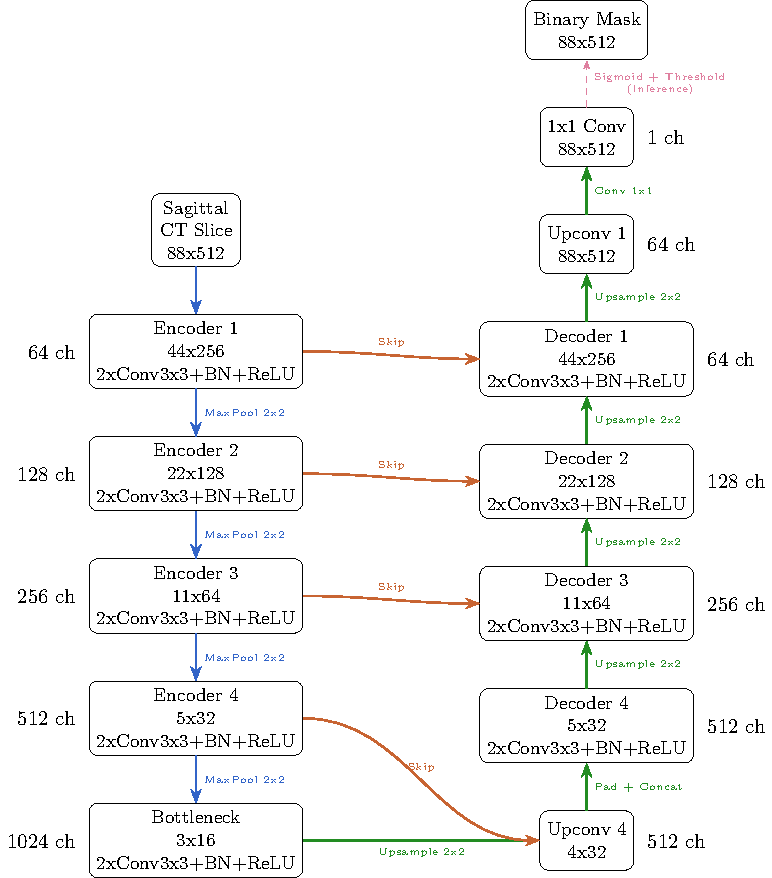
\includegraphics[width=0.8\textwidth,keepaspectratio]{unet.pdf}
    \caption{Architektur des U-Net-Modells für die Segmentierung von
    kV-CBCT-Bildern. Der kontrahierende Pfad (links) extrahiert Merkmale,
    während der expansive Pfad (rechts) präzise Segmentierungsmasken erzeugt.
    Skip-Connections verbinden die Pfade zur Erhaltung hochauflösender Details.}
    \label{fig:unet}
\end{figure}

\section{Ergebnisse}
Die Segmentierungsleistung wurde anhand des Dice-Koeffizienten, Präzision,
Recall und der Hausdorff-Distanz (HD) auf den Validierungsdaten bewertet.
Der Füllungszustand wird bewertet, indem die Höhe der binären Segmentierungsmasken
in Pixeln gemessen wird und mit den Ground-Truth-Masken verglichen wird. 

\begin{table}[H]
    \centering
    \scriptsize
    \begin{tabular}{p{1.8cm}p{2.8cm}p{1.8cm}p{1.8cm}p{3cm}}
      \toprule
      \textbf{Organ} & \textbf{Dice-Wert\newline (Mittel ± SD)} & \textbf{Präzision} & \textbf{Recall} & \textbf{Hausdorff-Distanz\newline (px, Mittel ± SD)} \\
      \midrule
      Harnblase & 0,9149 ± 0,0852 & 0,8974 & 0,9454 & 9,1419 ± 9,0216 \\
      Rektum & 0,7848 ± 0,1641 & 0,8019 & 0,7958 & 11,5230 ± 10,5643 \\
      \bottomrule
    \end{tabular}
    \caption{Segmentierungsmetriken auf Validierungsdaten (aggregiert über 5-Fold-Kreuzvalidierung).}
    \label{tab:results}
\end{table}

Die hohen Dice-Werte, Präzision und Recall sowie moderaten Hausdorff-Distanzen
zeigen eine zuverlässige Segmentierung, wobei die Harnblase präziser segmentiert
wurde als das Rektum, was auf dessen größere anatomische Variabilität
zurückzuführen ist.  Die Verlustkurven (Abb. \ref{fig:loss_curves}) zeigen, dass
beide Modelle eine stabile Konvergenz erreichen nach ca. 50 Epochen erreichen.

Die Segmentierungsleistung wird weiter durch Abbildung 
\ref{fig:val_bladder} und \ref{fig:val_rectum} illustriert, die rohe sagittale
Schnitte, Ground-Truth-Masken und Modellvorhersagen für jeweils 6 Patienten (3 mit 
akzeptablen Dice Werten, sowie die 3 mit den niedrigsten Dice Werten) in
den Validierungssets für die Harnblasen- und Rektummodelle gezeigt.
Für die Harnblase (Abb. \ref{fig:val_bladder}) sieht man ein Fehler in dem
Ground-Truth Maske bei P132 (dritte Reihe, mittleres Panel) als Ursache für
den niedrigen Dice Wert. Beim P050 ist der Kontrast schlecht - evtl. hat der
Patient gehustet während der Aufnahme, und die Kontrast zwischen Harnblase und
Darm ist gering, ebenfalls beim Patient P116.  Für das Rektum (Abb.
\ref{fig:val_rectum}) sind die Ground-Truth Masken augenscheinlich korrekt, auch
in den 3 Fällen schlechter Dice Werte. Beim Pat. P037 findet das Modell auch ein
Anteil des Rektums oberhalb der Ground-Truth Maske, was den Dice Wert
verringert, aber klinisch sinnvoll ist. Bei Patient P052 ist das Rektum kaum
abgebildet in der Ground-Trush Maske, und vom Modell nicht erkannt. Beim Patient
P129 ist die Modellvorhersage ggf. genauer an die anatomische Realität angepasst
als die Ground-Truth Maske, trotz Dice Wert von 0,62.

\begin{figure}[p]
    \centering
    \begin{subfigure}[b]{0.8\textwidth}
        \centering
        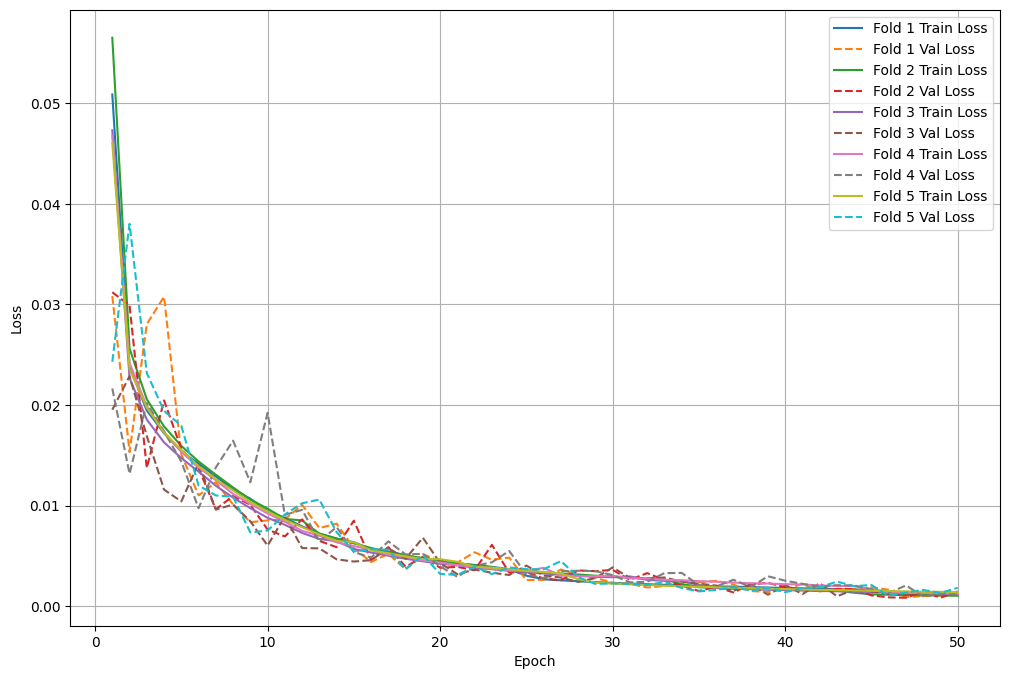
\includegraphics[width=\textwidth,keepaspectratio]{../images/bladder/loss_curves.png}
        \caption{Trainings- und Validierungsverluste für das Harnblasenmodell.}
        \label{fig:loss_curves_bladder}
    \end{subfigure}
    \vspace{0.5cm}
    \begin{subfigure}[b]{0.8\textwidth}
        \centering
        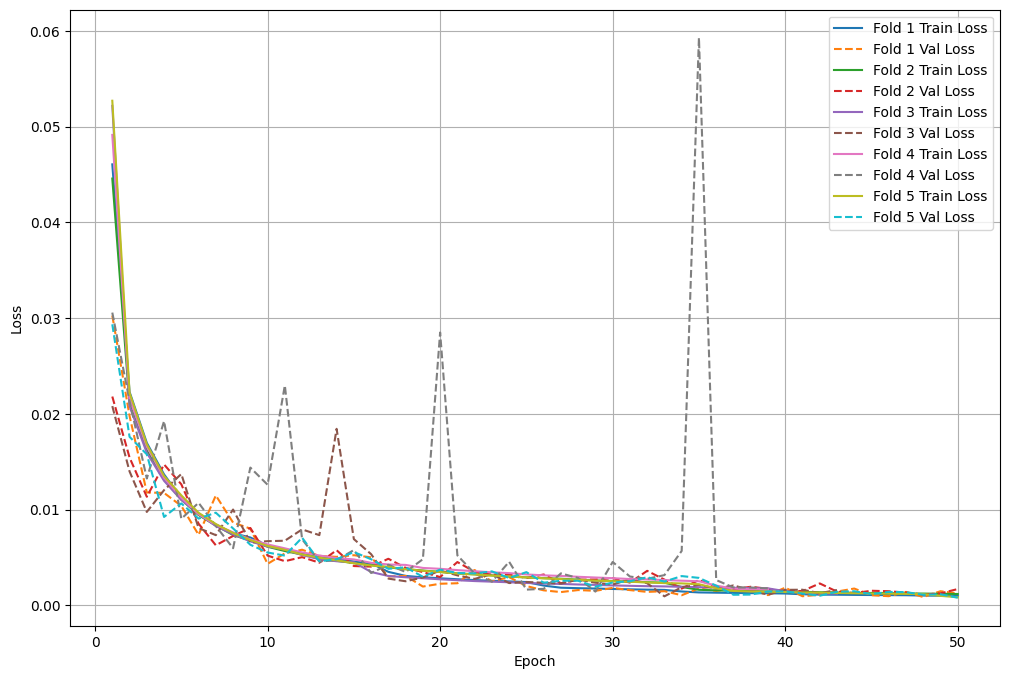
\includegraphics[width=\textwidth,keepaspectratio]{../images/rectum/loss_curves.png}
        \caption{Trainings- und Validierungsverluste für das Rektummodell.}
        \label{fig:loss_curves_rectum}
    \end{subfigure}
    \caption{Verlauf der Trainings- und Validierungsverluste über Epochen für die Harnblase und das Rektum, die die Konvergenz der Modelle zeigen.}
    \label{fig:loss_curves}
\end{figure}

\begin{figure}[p]
    \centering
    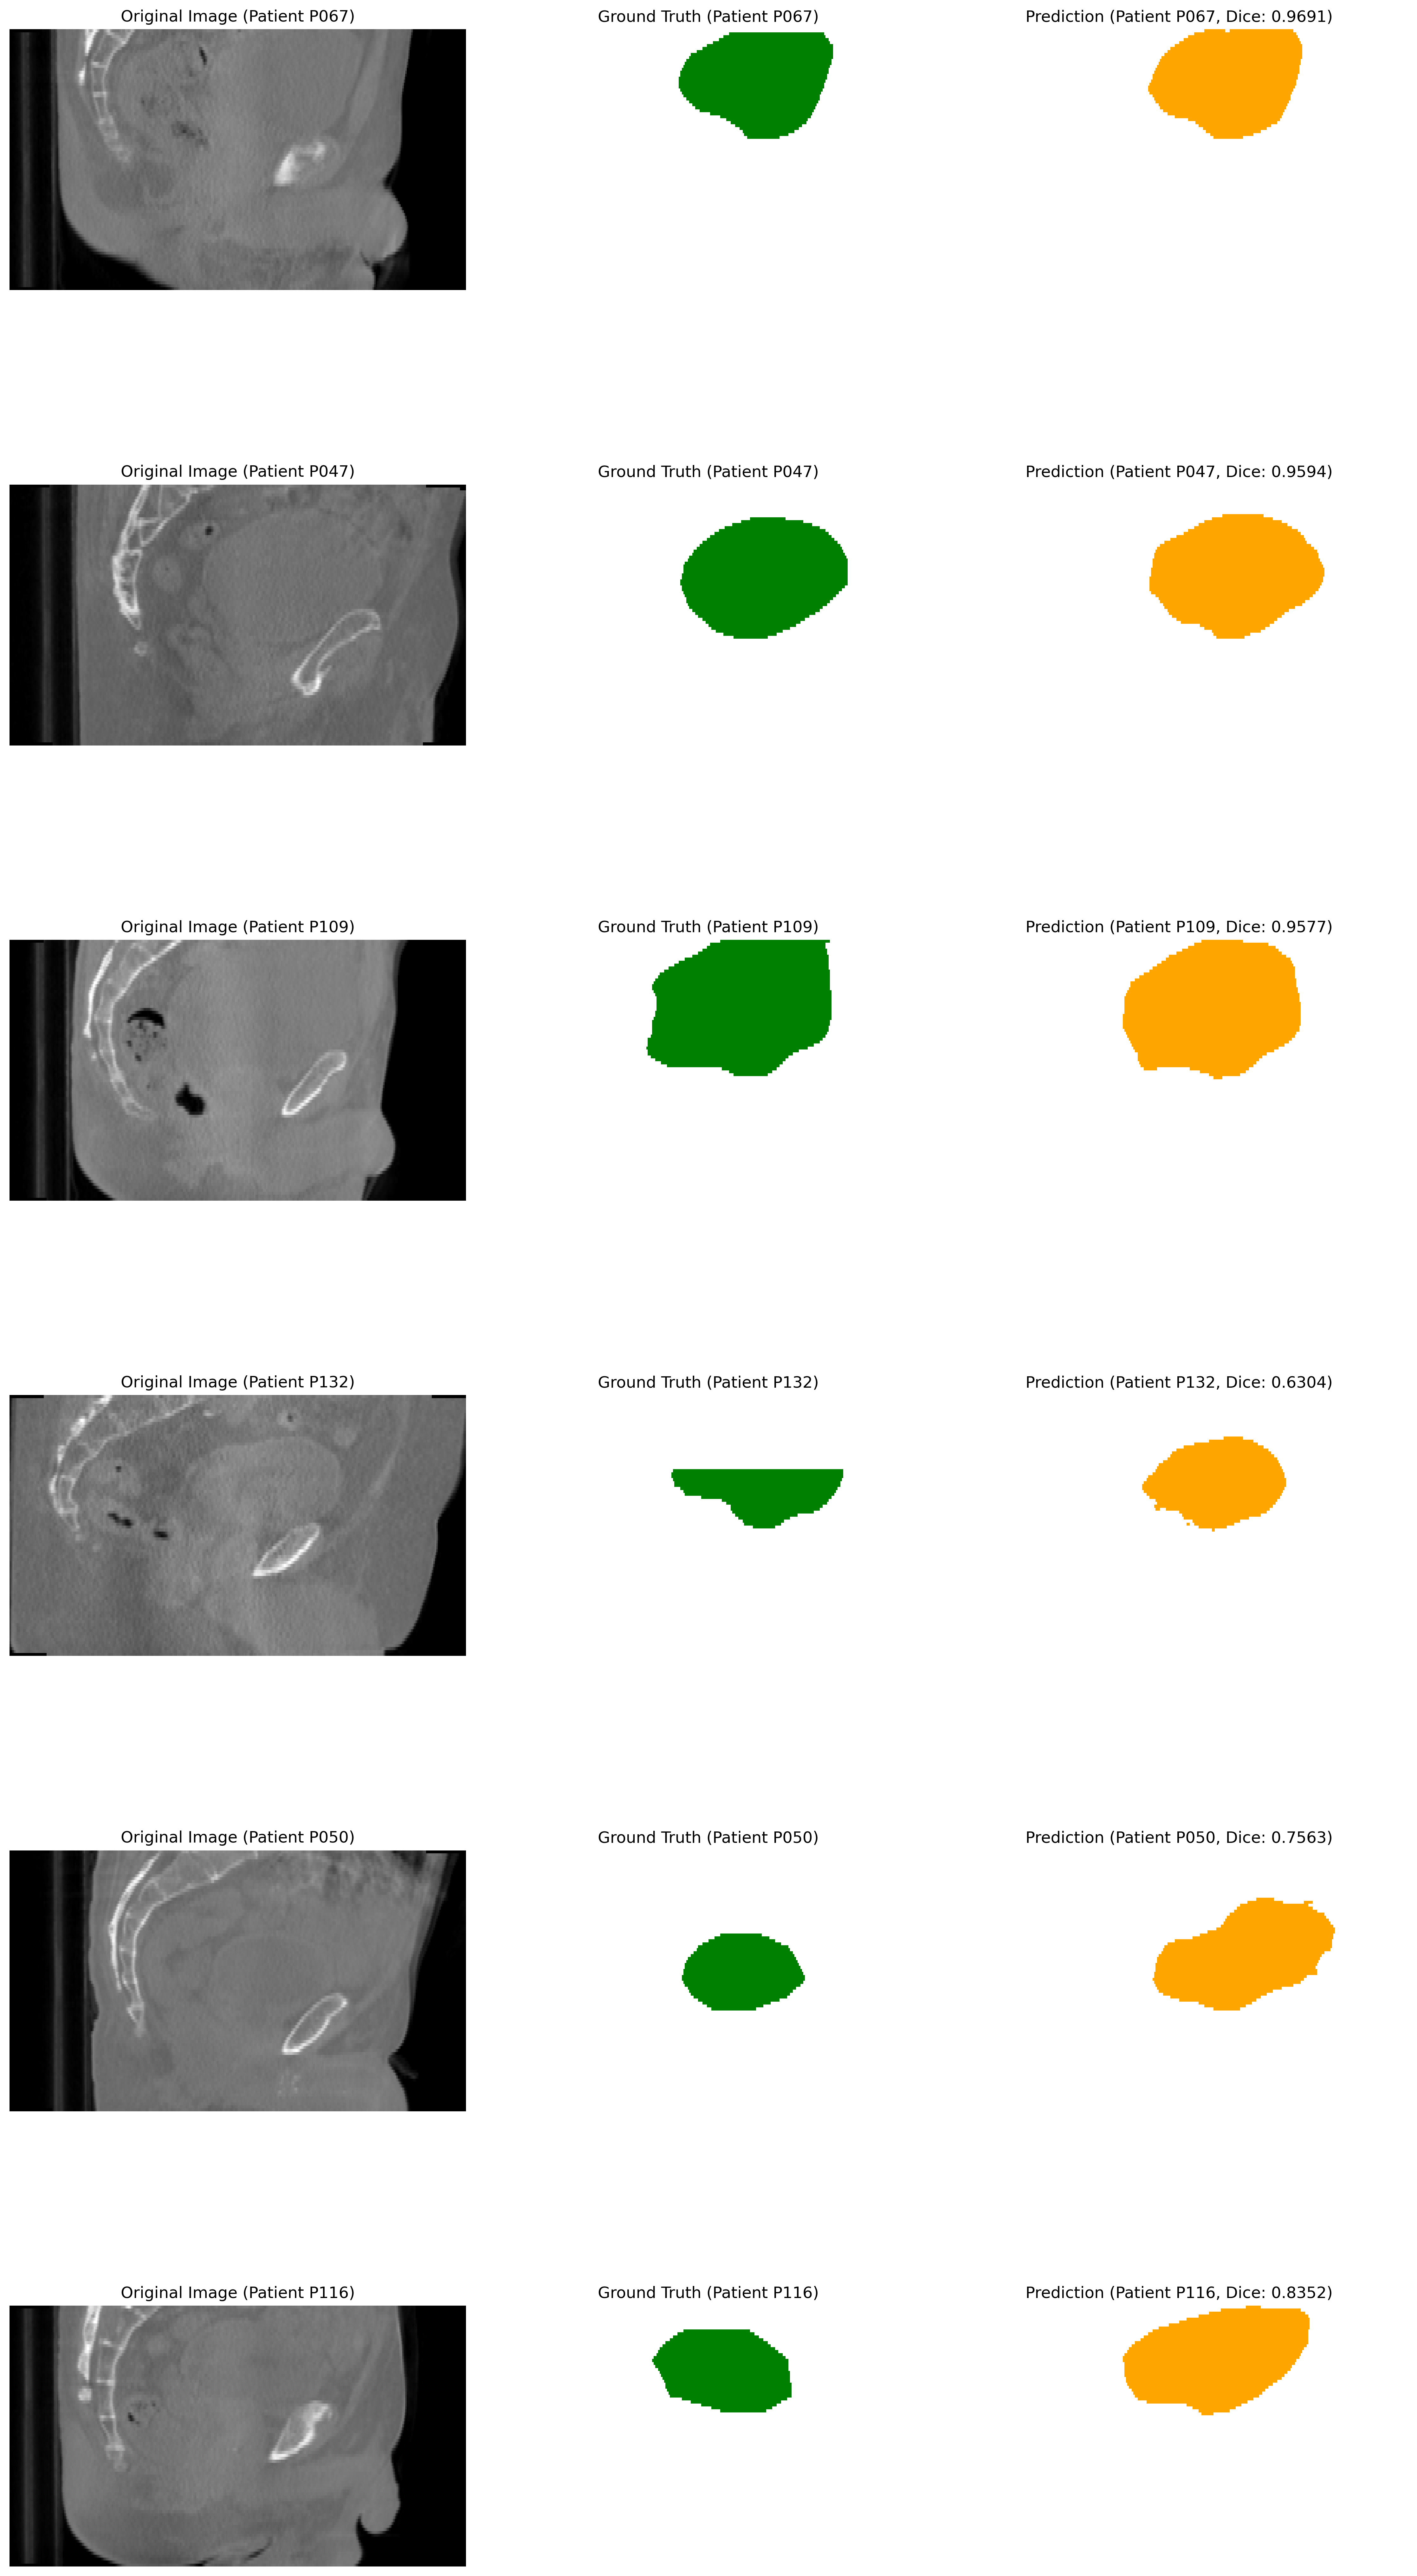
\includegraphics[height=0.9\textheight,keepaspectratio]{../images/bladder/segmentation_grid_6x3.png}
    \caption{Harnblase: Panels für Validierungspatienten (P067 - Dice 0.97,
    P047 - Dice 0.96, P109 - 0.96, P132 - Dice 0.63, P050 - Dice 0.76, P116 -
    Dice 0.84). Links: Originalschnitt; Mitte: Ground Truth (grün); Rechts:
    Vorhersage (orange).} \label{fig:val_bladder}
\end{figure}

\begin{figure}[p]
    \centering
    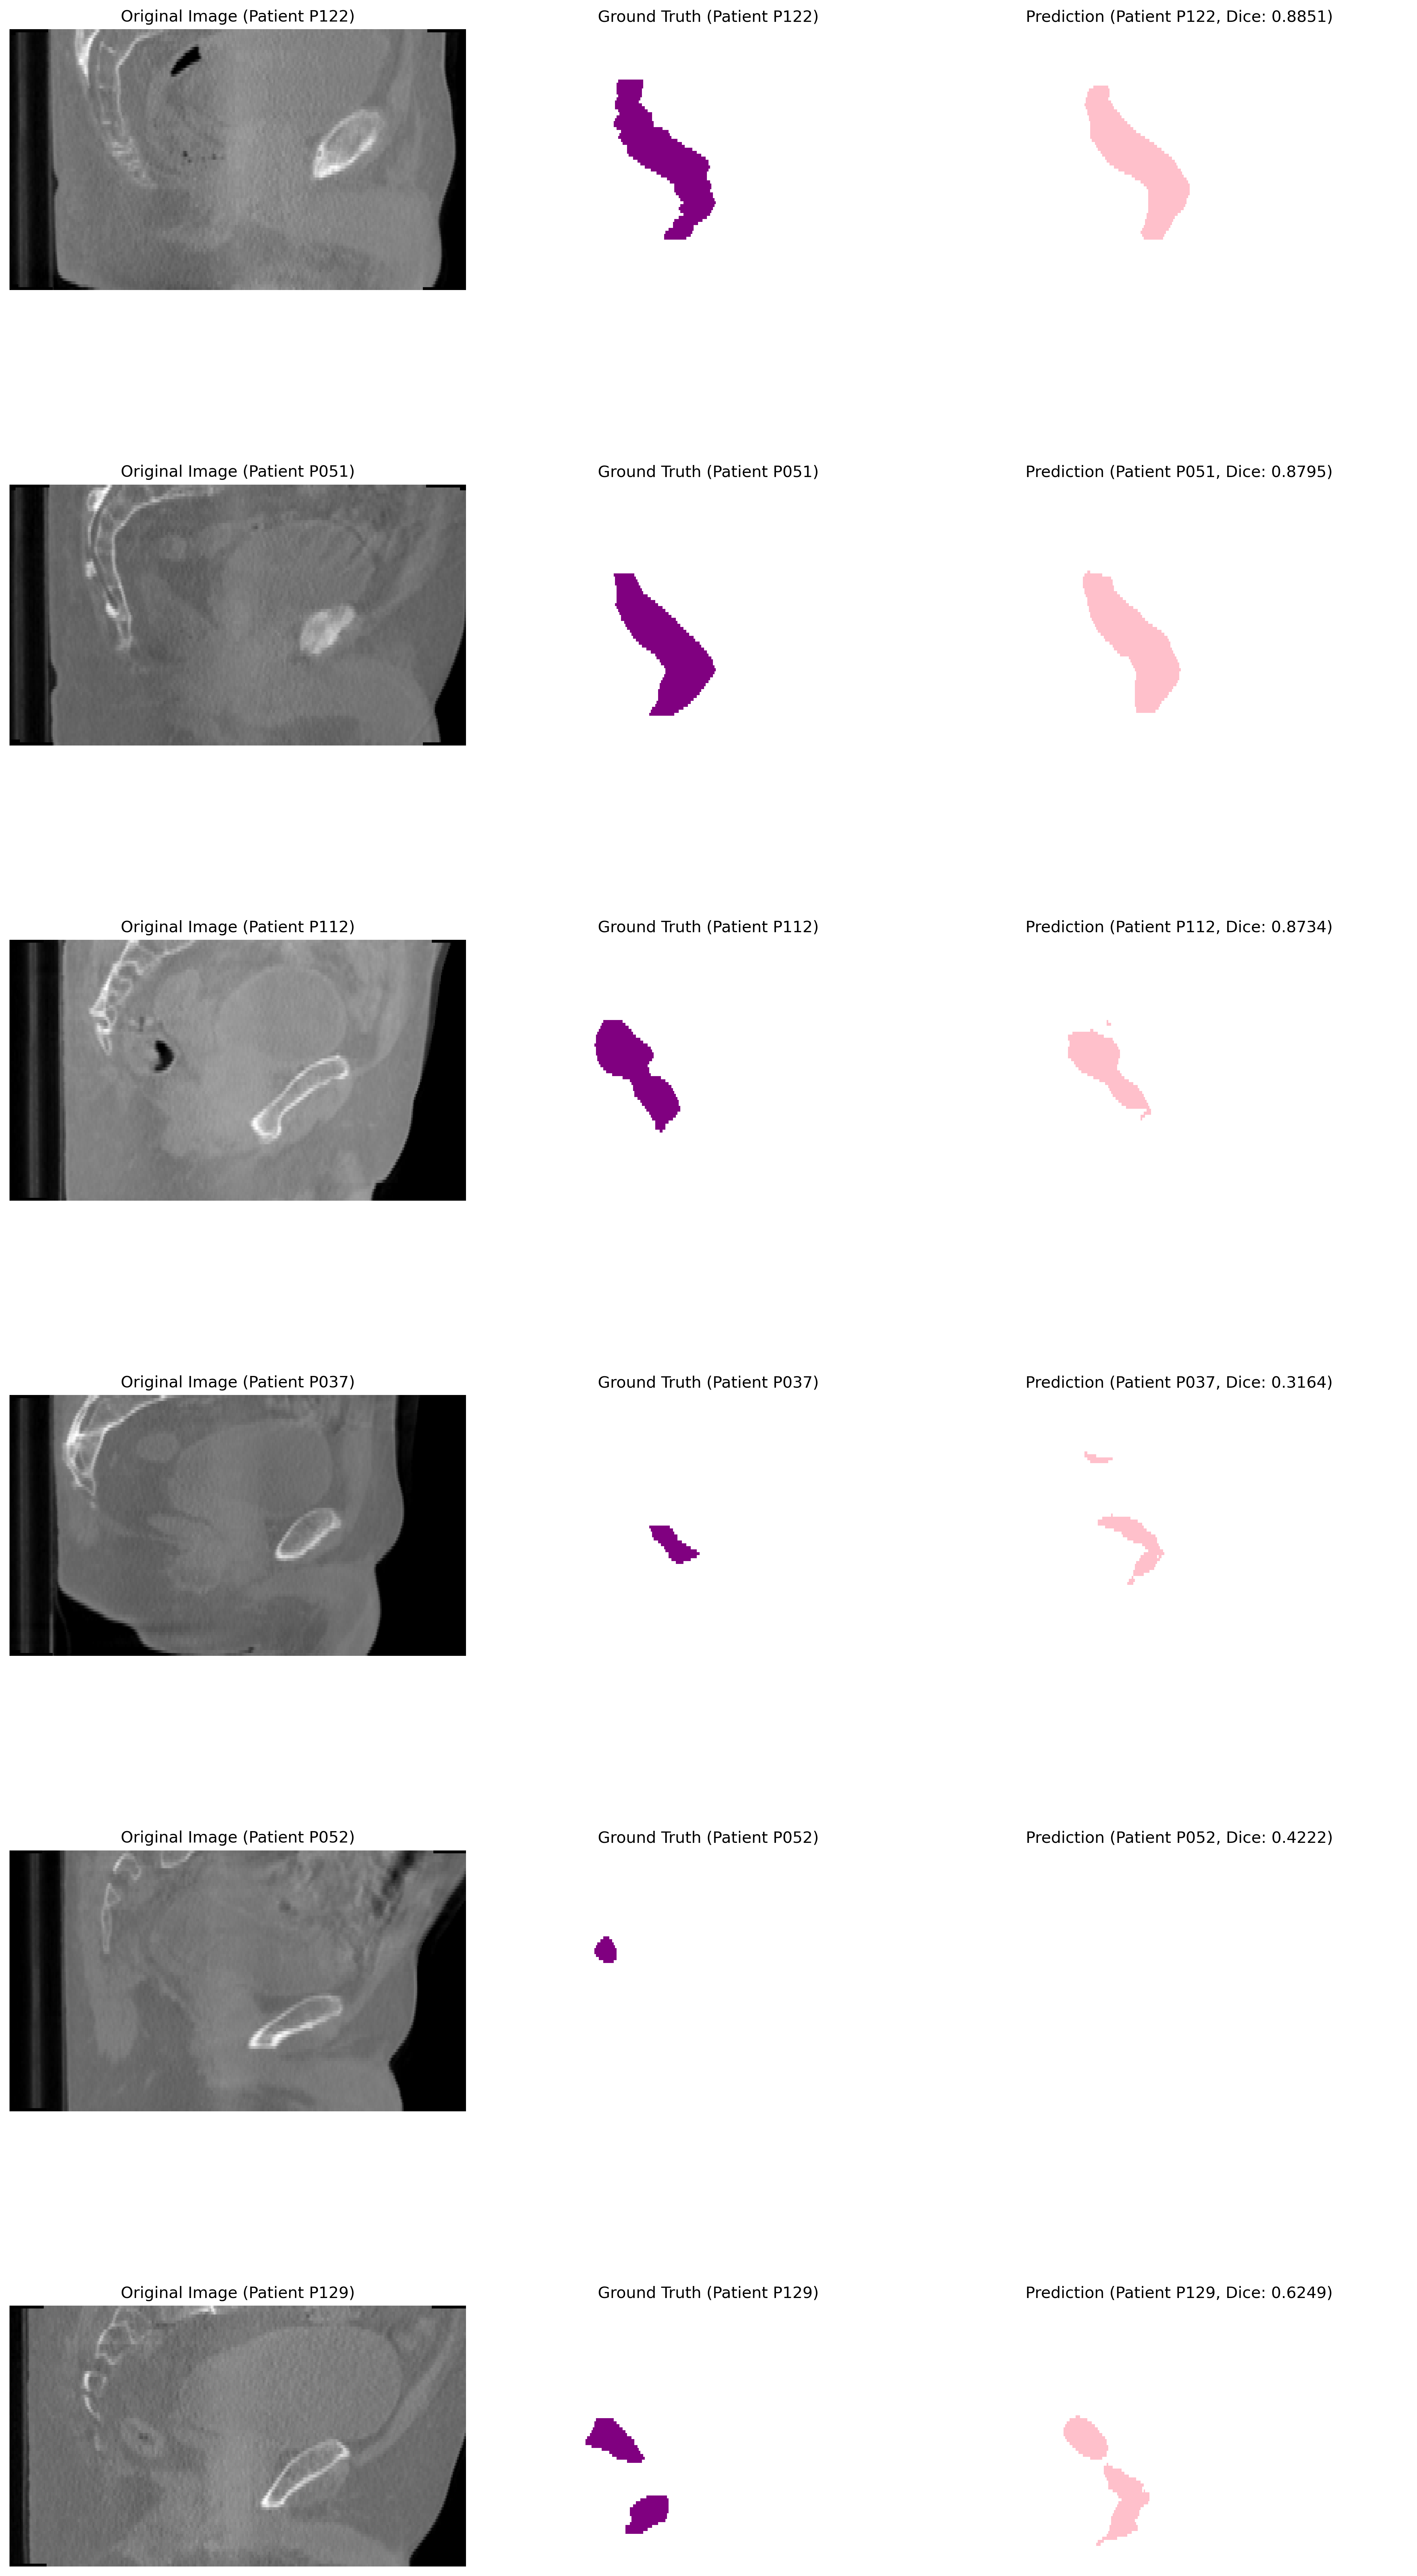
\includegraphics[height=0.9\textheight,keepaspectratio]{../images/rectum/segmentation_grid_6x3.png}
    \caption{Rektum: Panels für Validierungspatienten (P122 - Dice 0.89, P051 -
    Dice 0.88, P112 - Dice 0.87, P037 - Dice 0.31, P052 - Dice 0.42, P129 Dice
    0.62). Links: Originalschnitt; Mitte: Ground Truth (lila); Rechts:
    Vorhersage (pink).} \label{fig:val_rectum}
\end{figure}

\begin{figure}[p]
    \centering
    \begin{subfigure}[b]{0.8\textwidth}
        \centering
        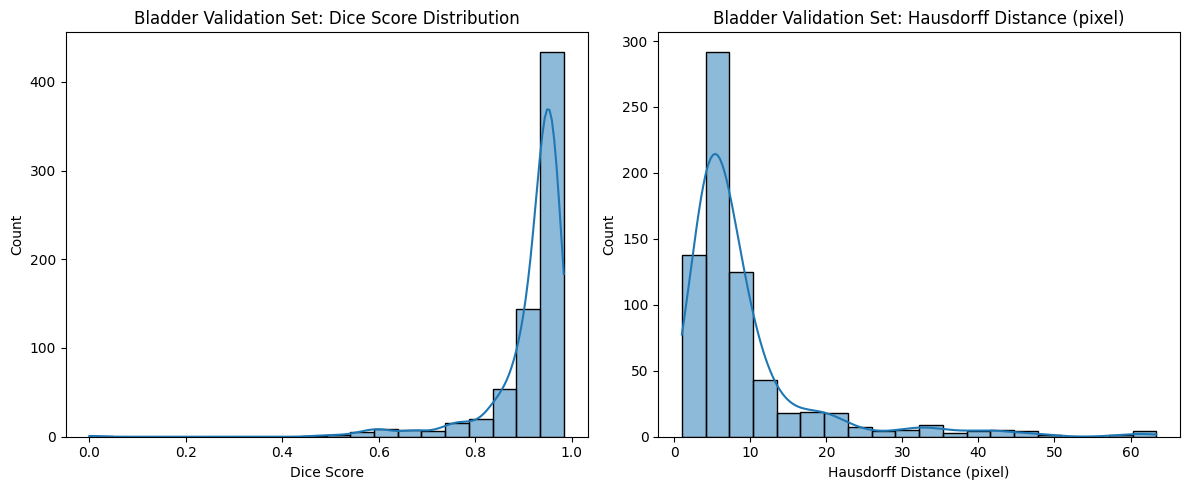
\includegraphics[width=\textwidth,keepaspectratio]{../images/bladder/val_metrics_distribution.png}
        \caption{Metrikenverteilung für die Harnblase (Dice und Hausdorff).}
        \label{fig:val_metrics_bladder}
    \end{subfigure}
    \vspace{0.5cm}
    \begin{subfigure}[b]{0.8\textwidth}
        \centering
        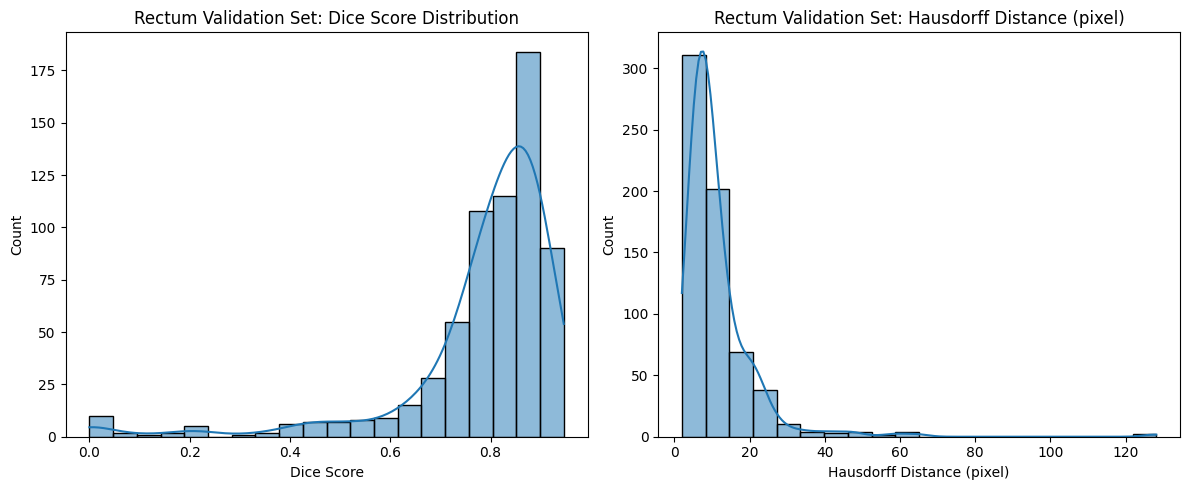
\includegraphics[width=\textwidth,keepaspectratio]{../images/rectum/val_metrics_distribution.png}
        \caption{Metrikenverteilung für das Rektum (Dice und Hausdorff).}
        \label{fig:val_metrics_rectum}
    \end{subfigure}
    \caption{Verteilung der Validierungsmetriken für Harnblase und Rektum.}
    \label{fig:val_metrics}
\end{figure}

\begin{figure}[p]
    \centering
    \begin{subfigure}[b]{0.8\textwidth}
        \centering
        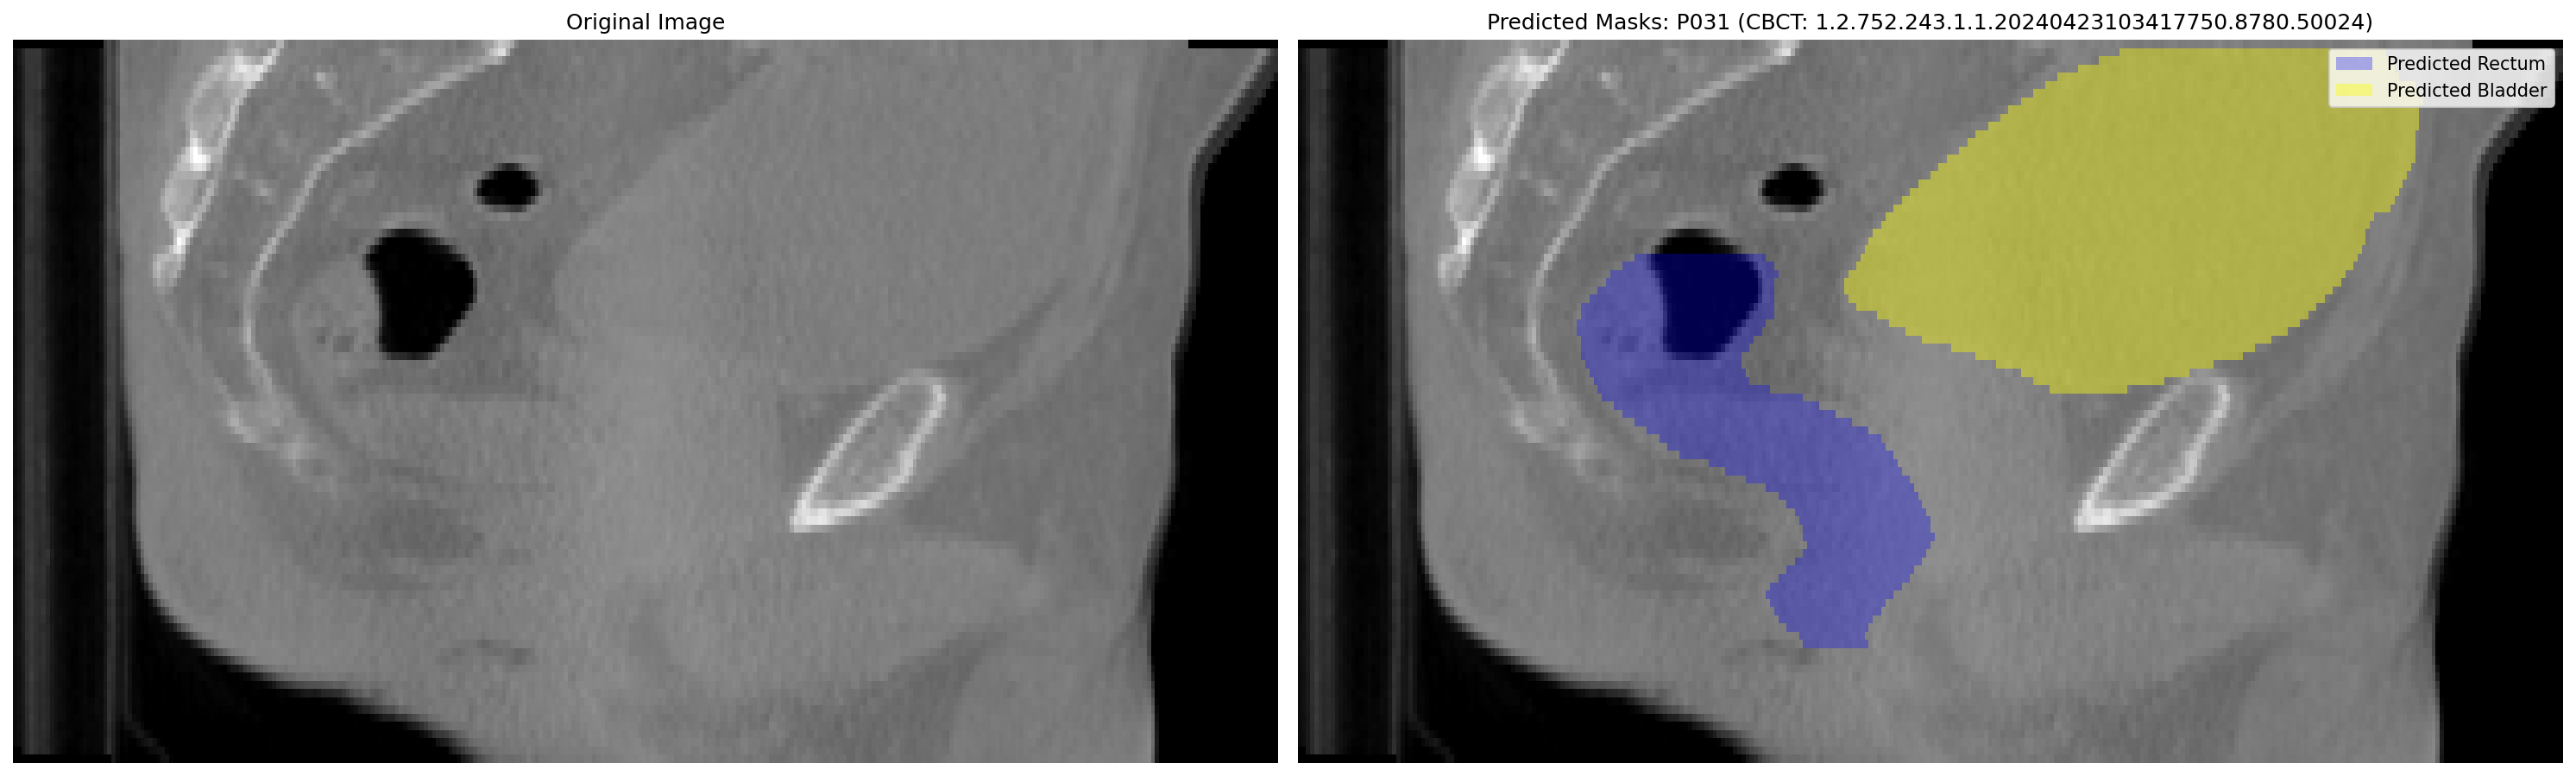
\includegraphics[width=\textwidth,keepaspectratio]{../images/predicted_masks_P031_1.2.752.243.1.1.20240423103417750.8780.50024.png}
        \caption{Überlagerte Vorhersagen für gemeinsamen Validierungspatienten (Patient 31, CBCT-ID: 1.2.752.243.1.1.20240423103417750.8780.50024).}
        \label{fig:predicted_overlays_p031}
    \end{subfigure}
    \vspace{0.5cm}
    \begin{subfigure}[b]{0.8\textwidth}
        \centering
        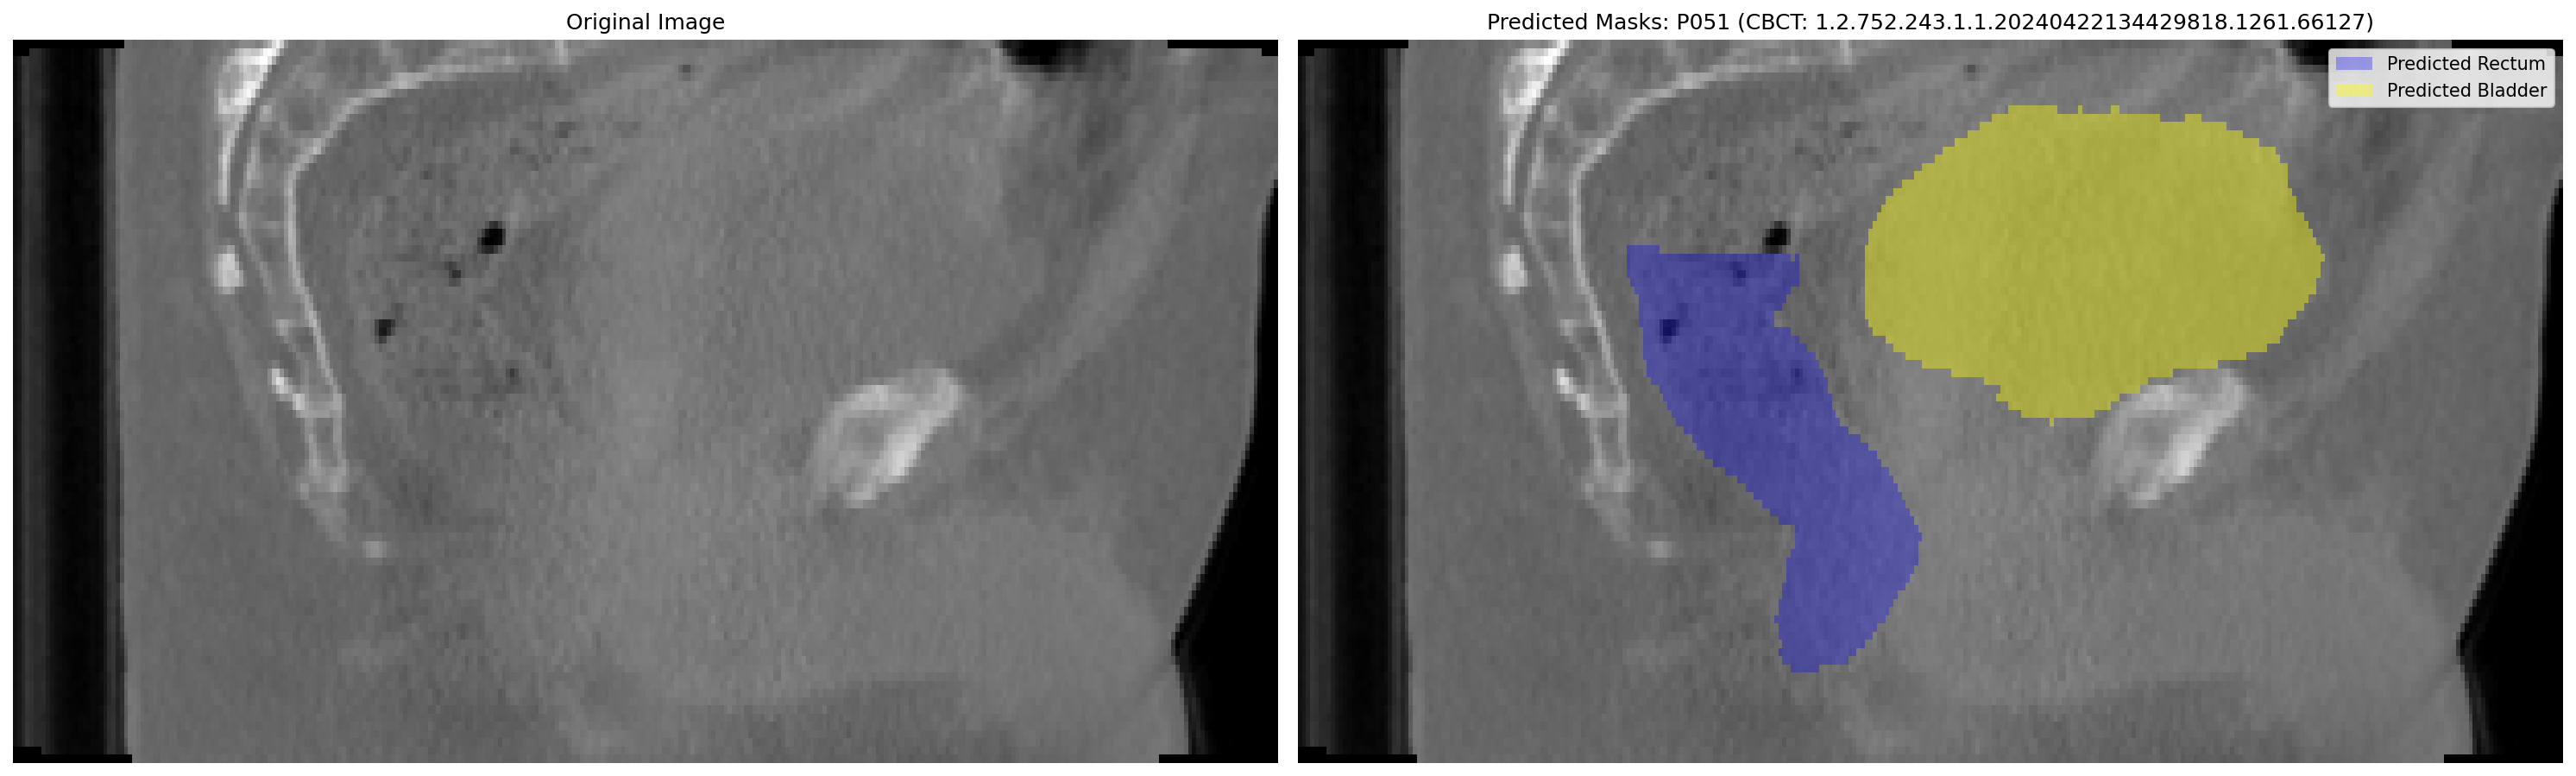
\includegraphics[width=\textwidth,keepaspectratio]{../images/predicted_masks_P051_1.2.752.243.1.1.20240422134429818.1261.66127.png}
        \caption{Überlagerte Vorhersagen für gemeinsamen Validierungspatienten (Patient 51, CBCT-ID: 1.2.752.243.1.1.20240422134429818.1261.66127).}
        \label{fig:predicted_overlays_p051}
    \end{subfigure}
    \vspace{0.5cm}
    \begin{subfigure}[b]{0.8\textwidth}
        \centering
        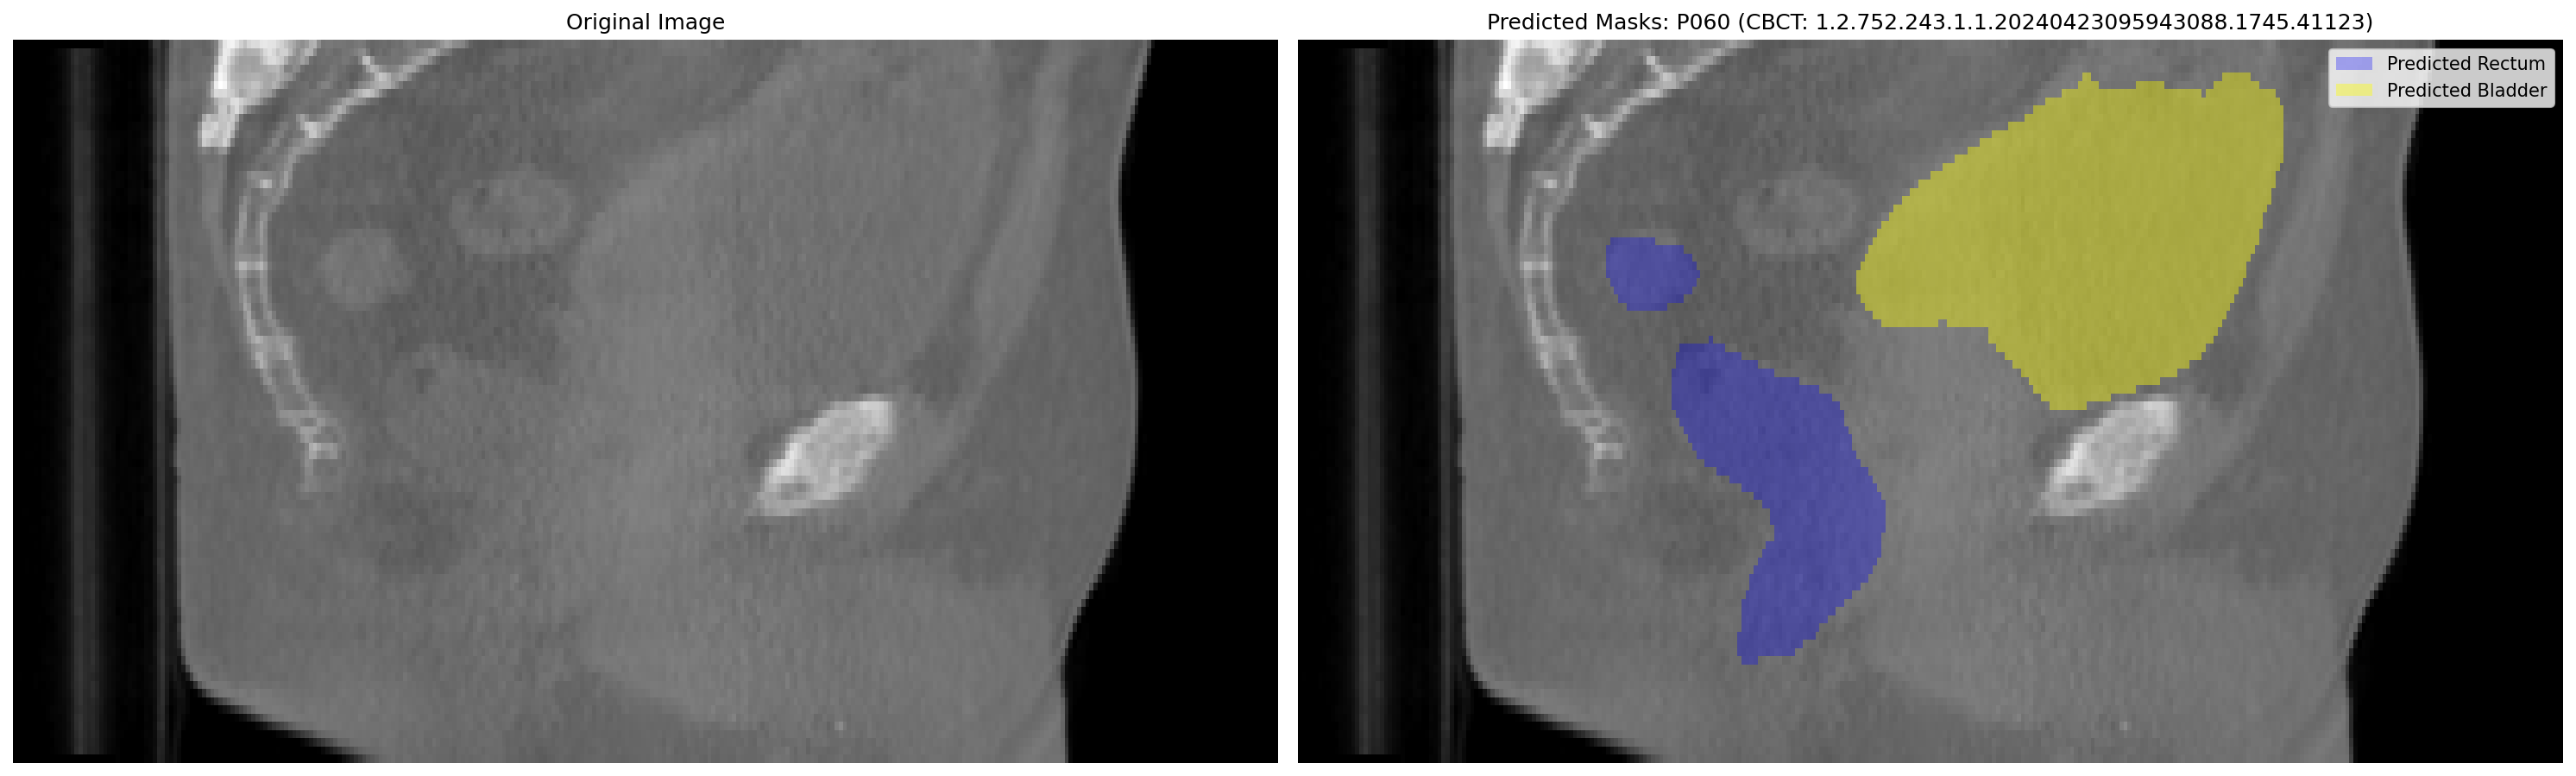
\includegraphics[width=\textwidth,keepaspectratio]{../images/predicted_masks_P060_1.2.752.243.1.1.20240423095943088.1745.41123.png}
        \caption{Überlagerte Vorhersagen für gemeinsamen Validierungspatienten (Patient 60, CBCT-ID: 1.2.752.243.1.1.20240423095943088.1745.41123).}
        \label{fig:predicted_overlays_p060}
    \end{subfigure}
    \caption{Überlagerte Modellvorhersagen für Harnblase (gelb) und Rektum (blau) beispielhaft auf gemeinsamen Validierungspatienten angewandt.}
    \label{fig:predicted_overlays}
\end{figure}

\section{Diskussion}
Die Methode ermöglicht eine präzise Segmentierung von Harnblase und Rektum. Der
Dice-Wert von 0,9149 ± 0,0852 für die Harnblase und 0,7848 ± 0,1641 für das
Rektum, kombiniert mit Hausdorff-Distanzen von 9,1419 ± 9,0216 px bzw. 11,5230 ± 10,5643 px,
liefert verlässliche Ergebnisse für den täglichen Einsatz in der IGRT. Die
höhere Standardabweichung beim Rektum spiegelt dessen größere anatomische
Variabilität wider \citep{rayed2024}. Die Verlustkurven (Abb. \ref{fig:loss_curves})
zeigen, dass beide Modelle eine stabile Konvergenz erreichen.

Die trainierten Modelle können auf einem herkömmlichen Computer in wenigen Sekunden
(nahezu in Echtzeit) ausgeführt werden, was eine Integration in den klinischen
Alltag, etwa als Plugin für das RayStation- oder Aria-System, ermöglicht und die
tägliche Überprüfung der Organlage bzw Füllung praktikabel macht \citep{antonelli2022}.

Zukünftig könnte die KI-basierte Segmentierung den Einsatz von Fiducials (z.B.
Goldmarker für die IGRT) in bestimmten Fällen ersetzen, was Behandlungskosten und
-zeit reduzieren sowie die mit invasiven Eingriffen verbundenen Risiken vermeiden
könnte.

Eine Erweiterung des Modells auf das gesamte kV-CBCT-Volumen würde eine
3D-Segmentierung der Risikoorgane ermöglichen und die Genauigkeit sowie Robustheit
der Methode steigern. Dies würde jedoch eine größere Datenbasis und
mehr Rechenleistung erfordern. Da das Training auf einem Heimcomputer durchgeführt
wurde, priorisierten wir 2D für Echtzeit-Inferenz (Sekunden pro Bild) und
klinische Machbarkeit. Zukünftige Arbeiten könnten 3D-Modelle testen.

Im Vergleich zu Studien wie \citep{radici2024}, die Dice-Werte von ~0,90 für die
Harnblase und ~0,85-~0,90 für das Rektum auf CBCT-Daten berichten, zeigt unser Modell
vergleichbare Leistung für die Harnblase (0,9149) und leicht geringere für das
Rektum (0,7848), trotz der Herausforderung durch 2D-Schnitte. Die geringeren
Dice-Werte für das Rektum könnten auf dessen komplexe Geometrie und Füllungs-
variationen zurückzuführen sein, wie auch in \citep{rayed2024} beobachtet.

Zukünftig könnte ein Multi-Organ-Modell getestet werden, um Überlappungen zu
vermeiden und Konsistenz zu steigern \citep{wasserthal2023}. Ein
Performance-Vergleich zwischen Einzel- und Multi-Organ-Modellen wäre wertvoll,
allerdings ist die Inference für beide Organe einzeln Sekundenschnell und die
VRAM Anforderungen gering. Somit können beide Modelle gleichzeitig auf
Consumer-Hardware betrieben werden - wie in Abb. \ref{fig:predicted_overlays}
gezeigt (Code dafür bei github einsehbar \cite{rhone_repo}).

Theoretisch geplant ist eine Warnung an dem MTRA abzugeben bei einer
signifikanten Abweichung der Modellvorhersage vom Ground-Truth Maske, 
z.Bsp. bei einer Höhenunterschied von > 10 Pixeln oder ein Flächenabweichung
von > 20\%. Ob eine Höhenabweichung oder Flächenabweichung klinisch relevanter ist,
und ab welcher Schwelle eine Warnung sinnvoll ist, müsste in zukünftigen Studien
evaluiert werden.

Schlechteste Resultate i.S. von Dice Werten
traten bei schlecht segmentierten Organen auf, verursacht durch anatomische
Variationen, z.B. trunkierte Bilder, schlechten Kontrast durch Bildartefakte
(z.B. Metallimplantate oder Bewegungen) oder unvollständige Organerfassung im
CT. Dies deutet auf Einschränkungen in der Generalisierbarkeit des Modells hin,
insbesondere bei extremen Füllungszuständen oder Bildartefakten. Die Analyse der
Worst-Case-Beispiele zeigt, dass das Modell in solchen Fällen zu Über- oder
Untersegmentierungen neigt, was durch erweiterte Augmentation oder Transfer
Learning in zukünftigen Iterationen adressiert werden könnte.

Einschränkungen der Methode umfassen die Abhängigkeit von konsistenten
kV-CBCT-Parametern sowie den Informationsverlust durch die Dimensionsreduktion auf
2D. Der Datensatz ist homogen (keine Hochrisikoprofile, Daten von einem Gerät:
Elekta Synergy-System, kV=120, mAs=650). Anatomische Besonderheiten wie
postoperative Zustände, übermäßiges Darmgas oder Implantate waren selten; die
Modell-Performance bei solchen Fällen war eingeschränkt, wie die
Worst-Case-Analyse zeigt. Externe Validierung ist essenziell, um die
Generalisierungsfähigkeit zu prüfen. Zukünftige Arbeiten könnten Transfer
Learning, erweiterte Augmentation oder ein nnU-Net einsetzen, um die Robustheit
gegenüber variablen Geräteigenschaften zu verbessern.

\section{Schlussfolgerung}
Die KI-basierte Methode automatisiert die Überprüfung der Füllung von Harnblase
und Rektum effektiv und bietet Potenzial zur Verbesserung der Behandlungsqualität
und Effizienz in der IGRT. Die hohen Performancemetriken und die stabile
Konvergenz der Modelle (Abb. \ref{fig:loss_curves}) untermauern die
verlässliche Segmentierung der Risikoorgane, was den Einsatz in der klinischen
Praxis unterstützt.

\section{Literaturverzeichnis}
\bibliographystyle{plainnat} 
\bibliography{references} 

\end{document}
